\documentclass{beamer}
\usetheme{CambridgeUS}
\usecolortheme{dolphin} 
\usepackage[utf8]{inputenc}
\usepackage[spanish]{babel}
\usepackage{graphicx}

\title[Tecnologia]
{IPv6}
\subtitle{}
\author[Grupo 1] 
{Ignacio P\'erez Laborda\\B\'arbara Mart\'inez}
\institute[UB--FTI] 
{
  Facultad de Tecnolog\'ia Inform\'atica\\
  Universidad de Belgrano
}
\date[\today] 

\renewcommand{\thefootnote}{\roman{footnote}}

\begin{document}

%1
\begin{frame}


\includegraphics[height=0.2\textheight]{ub2.jpg} \hspace*{6cm}

\includegraphics[height=0.19\textheight]{FTI.jpg}  
\\[-0.1cm]
\titlepage


\end{frame}

%2
\begin{frame}
\frametitle{Las falencias de IPv4}

\begin{enumerate}[$*$]

	\item Cupo limitado de direcciones asignables
	\item Falta de garant\'ias de seguridad,confiabilidad,movilidad y autenticidad
	\item Estos elementos podian incluirse mediante parches, pero a\'un as\'i no garantizaban el pleno desempeño de los mismos
	\item Si bien IPv4 posee un sistema de "servicios diferenciados"\footnote[1]{Diffserv: servicio que analiza varios flujos de datos en vez de conexiones únicas o reservas de recursos } no se garantizaba una calidad de servicio necesaria para cubrir la demanda actual en el mercado
\end{enumerate}

\end{frame}

%3
\begin{frame}
\frametitle{¿Qué es IPv6?}

Es la version 6 del protocolo de internet.La evolucion del IPv4 y es un protocolo que soporta mas direcciones ($2^{128}$).\vspace{0.3cm}
\par Se solucionan problemas de direccionamiento y no son necesarias técnicas como el NAT\footnote{NAT (Network Address Translation - Traducción de Dirección de Red)}
% es un mecanismo utilizado por routers IP para intercambiar paquetes entre dos redes que se asignan mutuamente direcciones incompatibles} para proporcionar conectividad a todos los ordenadores/dispositivos de nuestra red.
\end{frame}

%4
\begin{frame}
\frametitle{Comparación IPv4 vs IPv6}

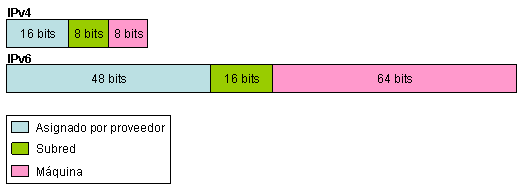
\includegraphics[scale=0.87]{estructura_direccion.png}

\end{frame}
%5

\begin{frame}
 \frametitle{Arquitectura de ipv6}
  \framesubtitle{\large{\vspace*{0,3cm}Principios de Comunicación\textbf{ Intranet}: \textbf{}}}
   \begin{itemize}
	\item IPv6 soporta una configuración automática integrada que dará en primer lugar una configuración sin estado y 	luego asignará el perfil indicado para cada situación
	\item Hoy en dia las direcciones MAC tienen 48 bits de longitud, ipv6 contará con direcciones mac de 64 bits
	\item Ipv6 cuenta con\textbf{ Neighbor Discovery} , un mecanismo para descubrir la presencia  de otros nodos en 		el mismo enlace
	%además de ver sus direcciones IP. Este protocolo también se ocupa de mantener limpios los caches donde se 	almacena la información relativa al contexto de la red a la que está conectado un nodo, este reemplaza al address solution protocol
	\item\textbf{ Path MTU Discover}: Servicio que permite al nodo fuente ver de antemano el tamaño del paquete 			mas grande que se puede enviar
%asi el paquete puede ser redimensionado antes de la transmision.Direcciones locales del sitio sólo se puede utilizar para las comunicaciones dentro del sitio. para
%comunicaciones más allá del sitio, las direcciones globales deben ser asignados con un más
%procedimiento de configuración automática escalable.
\end{itemize}
\end{frame}

%6
\begin{frame}
\frametitle{Arquitectura de ipv6}
 \framesubtitle{\large{\vspace*{0,3cm}Principios de Comunicación\textbf{ Internet} \textbf{}}}
  \begin{itemize}
	\item Al no tener un estado asignado, cada nodo es responsable de configurar su propia dirección
	%utilizando sus propias herramientas como el nd y el identificador de interfaces
	\item Autoconfiguracion con estado: es  una configuracion que depende de servidores que almacenarán datos en 		una base de datos \textbf{DHCPv6}.Sirve para administrar grandes redes
	%la autoconfiguración con estado proporciona
	%mayor escalabilidad a la hora de administrar grandes redes.
	%Autoconfiguración con estado puede ser utilizado simultáneamente con una sin estado

\end{itemize}
\end{frame}

%7
\begin{frame}
\frametitle{Arquitectura de ipv6}
\framesubtitle{\large{\vspace*{0,3cm}Principios de Comunicación Internet:\textbf{Red con estado}}}

Para entrar a una red de este tipo se debe enviar una solicitud de escucha a un servidor DHCPv6.Las ventajas de este tipo de conexión son
\begin{itemize}
	\item Control de distribucion y asignación
	\item Establecimiento de una jerarquía de direcciones
	\item Una fácil renumeración de las direcciones ante el cambio del proveedor de internet
	\item Se puede ejecutar un sistema con registro de host DHCPv6.
\end{itemize}
\end{frame}

%8
\begin{frame}
\frametitle{Ventajas del IPv6}

\begin{enumerate}[$*$]

	\item Mayor espacio de direccionamiento
	\item IPv6  incluye \textbf{IPsec}, que permite autenticación y encriptación del propio protocolo base
	\item IPv6 tiene una función de autoconfiguración en el protocolo base y de descubrir automáticamente el camino a internet\footnote{router discovery}
	\item Una característica obligatoria de IPv6 es la posibilidad de conexión y desconexión de nuestro ordenador de redes IPv6
	% y, por tanto, el poder viajar con él sin necesitar otra aplicación que nos permita que ese enchufe/desenchufe se pueda hacer directamente.
\end{enumerate}
\end{frame}

%9
\begin{frame}

\frametitle{Transicion de IPv4 a IPv6}

\begin{enumerate}[$*$]
	
	\item Se empezó con un protocolo sencillo con una cantidad de direcciones codificadas de 32 bits.
	 %Nunca pensaron que internet iba a tener un crecimiento tan descomunal
	%, de las cuales un grupo estaba reservado por paises como japon, eso acotaba aún mas la cantidad de direcciones disponibles.Nunca se llegó a usar toda la reserva de direcciones , así como tampoco se devolvieron los sobrantes
	\item Cada vez mas dispositivos empezaron a incluir servicios de conexión a internet
	% y cada vez había mas tráfico de datos en la red.\vspace{0.2cm}
	%,entonces  se empiezan a contemplar otros factores como por ejemplo, la seguridad y el aumento de la demanda.
	\item Desde hace tiempo se ha estado trabajando en el protocolo IPv6.\\ El problema radica en la transicion de un protocolo a otro, es un proceso que se hará de forma progresiva.
	%ciertas regiones latinoamerica todavía no tienen ipv6 configurado 
\end{enumerate}

\end{frame}

%10
\begin{frame}
\frametitle{Algunas empresas latinoamericanas que utilizan IPv6}

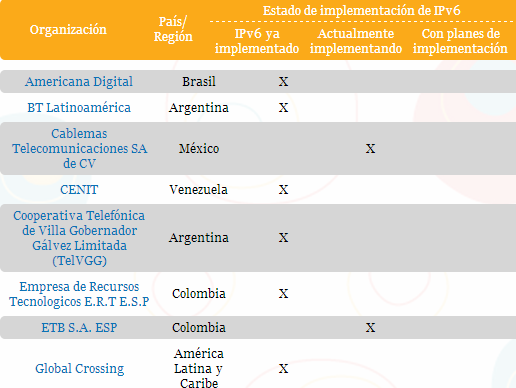
\includegraphics[height=1\textheight]{empresas_ipv6_la.png}

\end{frame}




\end{document}
